\documentclass{article}

% WMHS uses double-blind review. Do not add author-identifying information.
\usepackage[dblblindworkshop]{neurips_2026}
\workshoptitle{World Models for High-Stakes Health (WMHS)}

\usepackage[utf8]{inputenc}
\usepackage[T1]{fontenc}
\usepackage{hyperref}
\usepackage{url}
\usepackage{booktabs}
\usepackage{amsfonts}
\usepackage{nicefrac}
\usepackage{microtype}
\usepackage{xcolor}
\usepackage{graphicx}

\title{Cross-Dataset Generalization in 12-Lead ECG Classification}

\author{Anonymous Authors}

\begin{document}

\maketitle

\begin{abstract}
Deep learning models for automated ECG interpretation are typically trained and evaluated on a single dataset and show performance collapse when applied across datasets. We built a benchmark that trains and tests four architectures (InceptionTime, ResNet1D, a Transformer baseline, and the ECG-FM foundation model) across five public 12-lead ECG datasets (PTB-XL, CPSC2018, Georgia, MIMIC-IV-ECG, and CODE-15\%), and decomposes the resulting cross-dataset gaps into population, device, and label-schema shift components. ECG-FM achieved the highest mean in-distribution macro-AUROC (0.972), whereas ResNet1D achieved the highest mean cross-dataset macro-AUROC (0.924) and the smallest generalization gap (0.042). The raw performance gaps did not differ significantly across the shift groups, so we treat the weighted attribution as a sensitivity analysis rather than evidence that label-schema differences caused a specific percentage of the performance loss. A post-hoc normal-versus-abnormal analysis across all four architectures reduced the matched-record average generalization gap from 0.049 to 0.038, a reduction of 22.5\%. Alternative endpoint mappings changed absolute cross-dataset AUROC but did not change the model ranking.
\end{abstract}

\section{Introduction}

Deep learning models for 12-lead electrocardiogram (ECG) interpretation frequently approach cardiologist-level performance on held-out test data drawn from their training institutions, yet degrade in well-documented ways once deployed in new environments. These drops matter clinically: a classifier is only useful if it performs reliably on the hospital, hardware, and patient population it was not trained on. Cross-site evaluations typically attribute this degradation to a single undifferentiated construct, distribution shift, which in fact conflates at least three distinct mechanisms. Population shift arises because patient demographics (age, comorbidity burden, disease prevalence) differ across sites, producing base-rate miscalibration. Acquisition shift arises because differences in recording hardware, sampling rate, filtering, and record duration cause identical cardiac events to yield dissimilar signals. Label-schema shift arises because incompatible diagnostic vocabularies across sources cause clinical findings to be encoded, subdivided, or omitted inconsistently.

These three mechanisms call for different remedies. Recalibration addresses population shift; preprocessing or augmentation addresses acquisition shift; neither addresses label-schema shift. An aggregate performance metric cannot indicate which remedy is warranted, since it reports only the combined effect of all three, leaving a practitioner no way to decide whether the fix is recalibration, better preprocessing, or a corrected label mapping.

Label-schema shift has received the least scrutiny of the three, largely because harmonization is conventionally treated as invisible preprocessing. Source-to-target code mappings are typically built once, described in a single sentence, and left unpublished, which conceals decisions that materially change measured results. PTB-XL and the Georgia database, for instance, encode right bundle branch block under opposite members of a synonymous SNOMED code pair, so an arbitrary mapping choice can silently empty a class. Sinus rhythm and normal ECG likewise denote distinct concepts that differ by thousands of records in PTB-XL, yet some datasets encode only the latter. Each of these is a modeling decision, not a preprocessing step, and each changes the shift that is ultimately measured. Because the mapping is rarely published in full, two groups working from the same source datasets can report different cross-dataset gaps without either being aware that their harmonization choices, not their models, are the source of the disagreement.

We introduce a cross-dataset generalization benchmark for 12-lead ECG classification that decomposes observed performance drops into population, acquisition, and label-schema components rather than reporting them as a single aggregate figure. The benchmark draws on five public datasets spanning four continents: PTB-XL (Germany), CPSC2018 (China), the Georgia 12-lead Challenge database (United States), MIMIC-IV-ECG (United States), and CODE-15\% (Brazil). These sources differ in patient population, recording hardware, and native labeling schema, letting us hold two of the three shift mechanisms fixed while isolating the third.

This work makes four contributions. First, we release the complete label mapping as a versioned, citable artifact, in which every source code carries a rule identifier, every exclusion has a written rationale, and ambiguous codes record their rejected alternatives, so the mapping can be audited rather than taken on faith. Second, we show that the diagnostic classes expressible across all four schemas represented in this benchmark form a strict set intersection of exactly five members, and we document what information is lost at its boundaries. Third, we provide a protocol that isolates the three shift components instead of collapsing them into a single aggregate gap, reporting the attribution alongside a sensitivity analysis rather than as fixed ground truth. Fourth, we test whether the cross-dataset results and model rankings remain stable under a post-hoc normal-versus-abnormal analysis and three alternative endpoint mappings.

The datasets are available through public repositories, subject to their individual access requirements. The released pipeline documents the preprocessing, training, evaluation, and sensitivity-analysis steps required to reproduce the benchmark.

\section{Related work}

Public ECG benchmarking currently focuses on within-dataset evaluation, and the datasets themselves are the source of the label-schema problem that our benchmark measures. PTB-XL utilized the SCP-ECG coding standard for its 21,000+ recordings (Wagner et al., 2020), whilst other datasets like CPSC2018 and the Georgia 12-lead database exist under the SNOMED-CT schema (Alday et al., 2020). These schemas were independently defined and were not designed to be comparable with one another, leading to scenarios where the same diagnosis may have different coding standards. This is why a unified five-class mapping across four coding systems is more complex than it lets on.

When cross-dataset evaluation has occurred, a performance drop can occur, yet no diagnosis has been given as to why such events occur. This is particularly relevant in the case of Cardioformer, which performed excellently when trained and tested on MIMIC-IV, achieving a 96.3\% AUROC; however, when that same trained model was evaluated on PTB, the accuracy plummeted to 49.2\% AUROC (Mobin et al., 2025). The closest prior attempt at identifying this gap is BenchMD, which constructs a cross-dataset ECG evaluation using PTB-XL as a training source against Chapman-Shaoxing, Georgia, and CPSC2018 as targets, and explicitly mentions demographic and device-collection differences as the source behind the accuracy gap (Wantlin et al., 2023). BenchMD does mention categories that contribute to this gap, yet fails to quantify the extent to which these categories contribute. Additionally, it fails to consider label-schema shift despite pairing datasets with incompatible native coding systems. This project extends BenchMD's categories into the analytical core of a benchmark---a directional train/test matrix with per-cell shift attribution---rather than simply a qualitative observation.

% TODO(citations): Verify the exact Berger et al. (2026) bibliography entry.
A recent position paper argues that ECG benchmarking is dysfunctional. This was shown through Berger et al. (2026), where it was found that models with random, untrained weights performed nearly as well as state-of-the-art pretrained models on several standard tasks. This finding indicates that the structure of current tests is designed poorly. Their findings are adjacent to what this project focuses on; however, there is a distinct difference in that Berger et al. broaden what is being evaluated; however, our project analyzes why performance degrades when training and testing sources diverge.

% TODO(citations): Verify the exact Zhou et al. (2026) ECG-FM bibliography entry.
Foundation models introduce a further complication for what counts as genuinely held-out evaluation. ECG-FM is pretrained on the PhysioNet Challenge 2021 dataset and MIMIC-IV-ECG, and because Challenge 2021 itself incorporates PTB-XL, CPSC2018, and Georgia, this pretraining overlaps with three of this benchmark's five source datasets. Zhou et al. (2026) explicitly flag that this overlap limits ECG-FM's validity as an independently evaluated model on PTB-XL. This benchmark treats that overlap as an empirical question to audit, not an assumption, before comparing ECG-FM's in-distribution performance against from-scratch architectures.

No existing work pairs the five major public 12-lead ECG datasets in a directional train/test matrix with each cross-dataset cell attributed to a specific, quantified combination of population, device, and label-schema shift. That is this project's contribution.

\section{Methods}

\paragraph{Datasets.}
We use PTB-XL (21,837 records, Germany), a 50,000-record subsample of MIMIC-IV-ECG (United States), the Georgia 12-lead ECG Challenge database (10,344 records, United States), CPSC2018 (6,877 records, China), and a 50,000-record stratified subsample of CODE-15\% (Brazil). Together, these sources span four distinct labeling schemas: SCP-ECG statements, SNOMED-CT concept identifiers, a nine-class integer scheme, and a six-label boolean scheme.

\paragraph{Label harmonization.}
Because CPSC2018 and CODE-15\% rely on closed vocabularies, the set of classes natively representable across all sources is their intersection, which yields five members: normal sinus rhythm, atrial fibrillation or flutter, first-degree atrioventricular block, left bundle branch block, and right bundle branch block. We map every source code to these classes using an explicit rule typology distinguishing direct assignment, merge, proxy, and derivation. Normal sinus rhythm is provided in two variants, one defined as sinus rhythm and the other as normal ECG, as no single definition is native to all schemas. The complete mapping, including its exclusions and unresolved ambiguities, is released alongside this work.

\paragraph{Models and splits.}
We evaluate InceptionTime, ResNet1D, a vanilla Transformer, and ECG-FM on the harmonized five-class multi-label task. The first three architectures are trained from scratch, whereas ECG-FM uses its pretrained backbone with the study-specific adapter. Splits are constructed at the patient level where identifiers permit, stratified on the rarest class rather than drawn at random, and constrained to guarantee a minimum number of positive examples per class per evaluation fold. MIMIC-IV-ECG and CODE-15\% are subsampled with stratification rather than uniformly so as to preserve their class composition.

\paragraph{Evaluation.}
We report macro-AUROC and per-class AUROC for each source-to-target evaluation. Population, device, and label-schema indicators are recorded for every ordered dataset pair, while the composite shift score is reported as a sensitivity analysis rather than fixed ground truth. We conducted the revision analyses post hoc using the saved five-class predictions, without retraining the models. For the normal-versus-abnormal analysis, the four abnormal-class probabilities were combined and evaluated on the same eligible records as the five-class task. For the mapping sensitivity analysis, we tested an exclusive definition of normal, removed the ambiguous normal class, and combined LBBB and RBBB into a single bundle branch block class.

\begin{figure}[t]
  \centering
  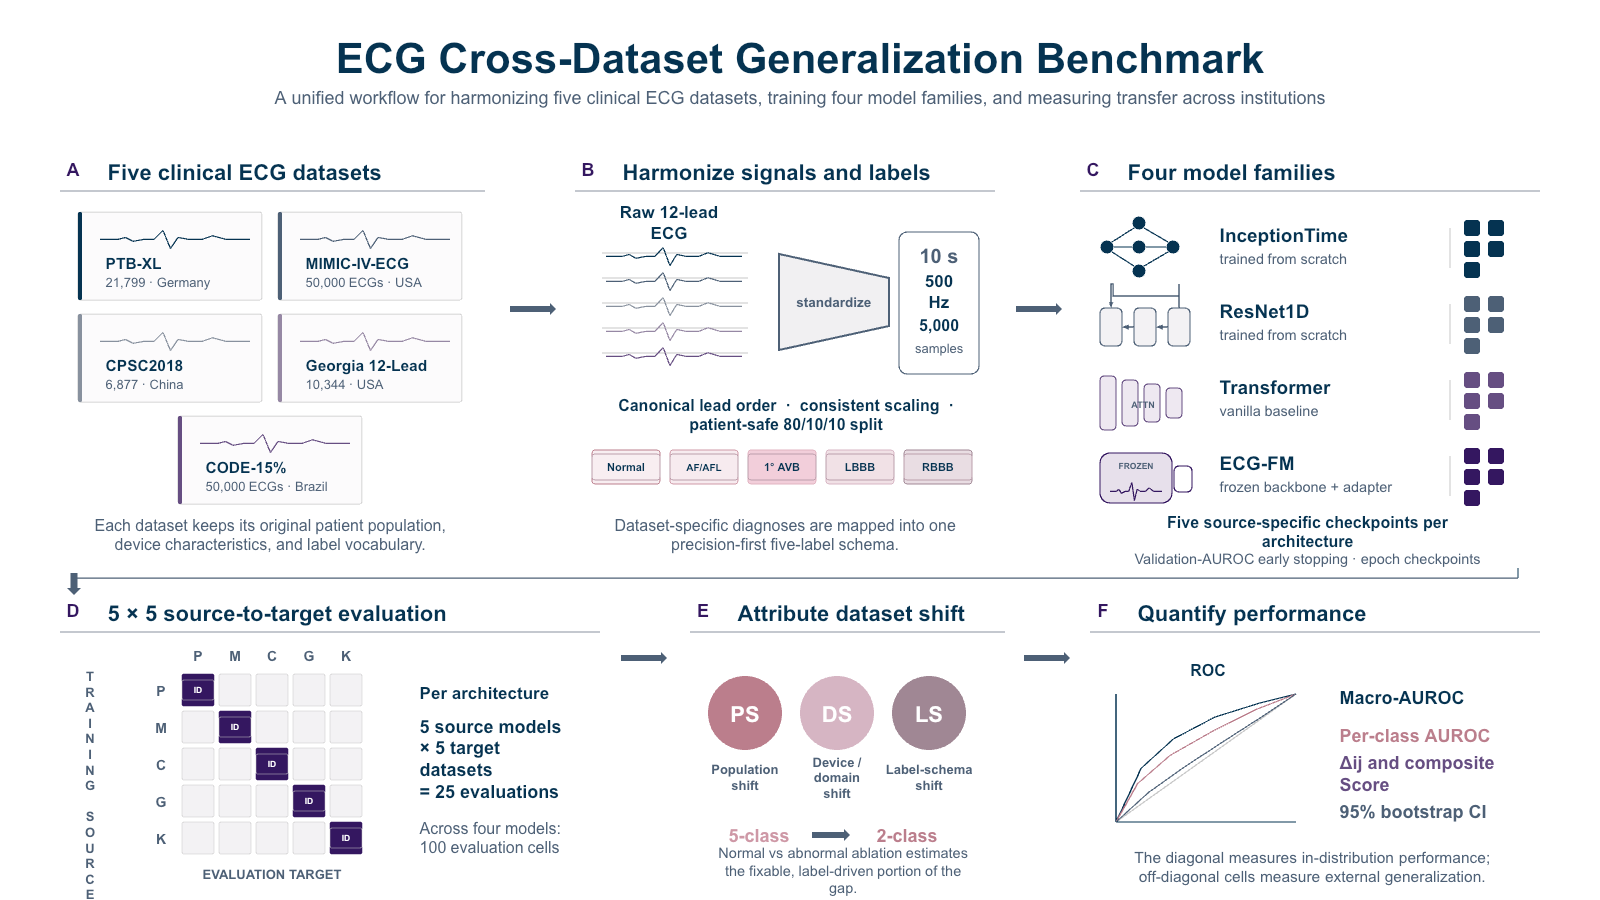
\includegraphics[width=\linewidth]{figures/fig1_methods_pipeline.png}
  \caption{Benchmark workflow. Five ECG datasets are harmonized to a shared signal and label contract, used to train four model families, and evaluated in a complete directional source-to-target matrix. Population (PS), device (DS), and label-schema (LS) indicators characterize each transfer cell.}
  \label{fig:pipeline}
\end{figure}

\section{Results}

Our results show that in-distribution performance does not predict cross-dataset performance. ECG-FM achieved the highest mean in-distribution macro-AUROC (0.972), followed by ResNet1D (0.966), InceptionTime (0.965), and the Transformer (0.937). The ordering changed under external evaluation: ResNet1D achieved the highest mean cross-dataset macro-AUROC (0.924) and smallest gap (0.042), followed by InceptionTime (0.919; gap 0.046), ECG-FM (0.888; gap 0.085), and the Transformer (0.879; gap 0.058). Figure~\ref{fig:matrices} shows the complete directional matrices.

\begin{figure}[t]
  \centering
  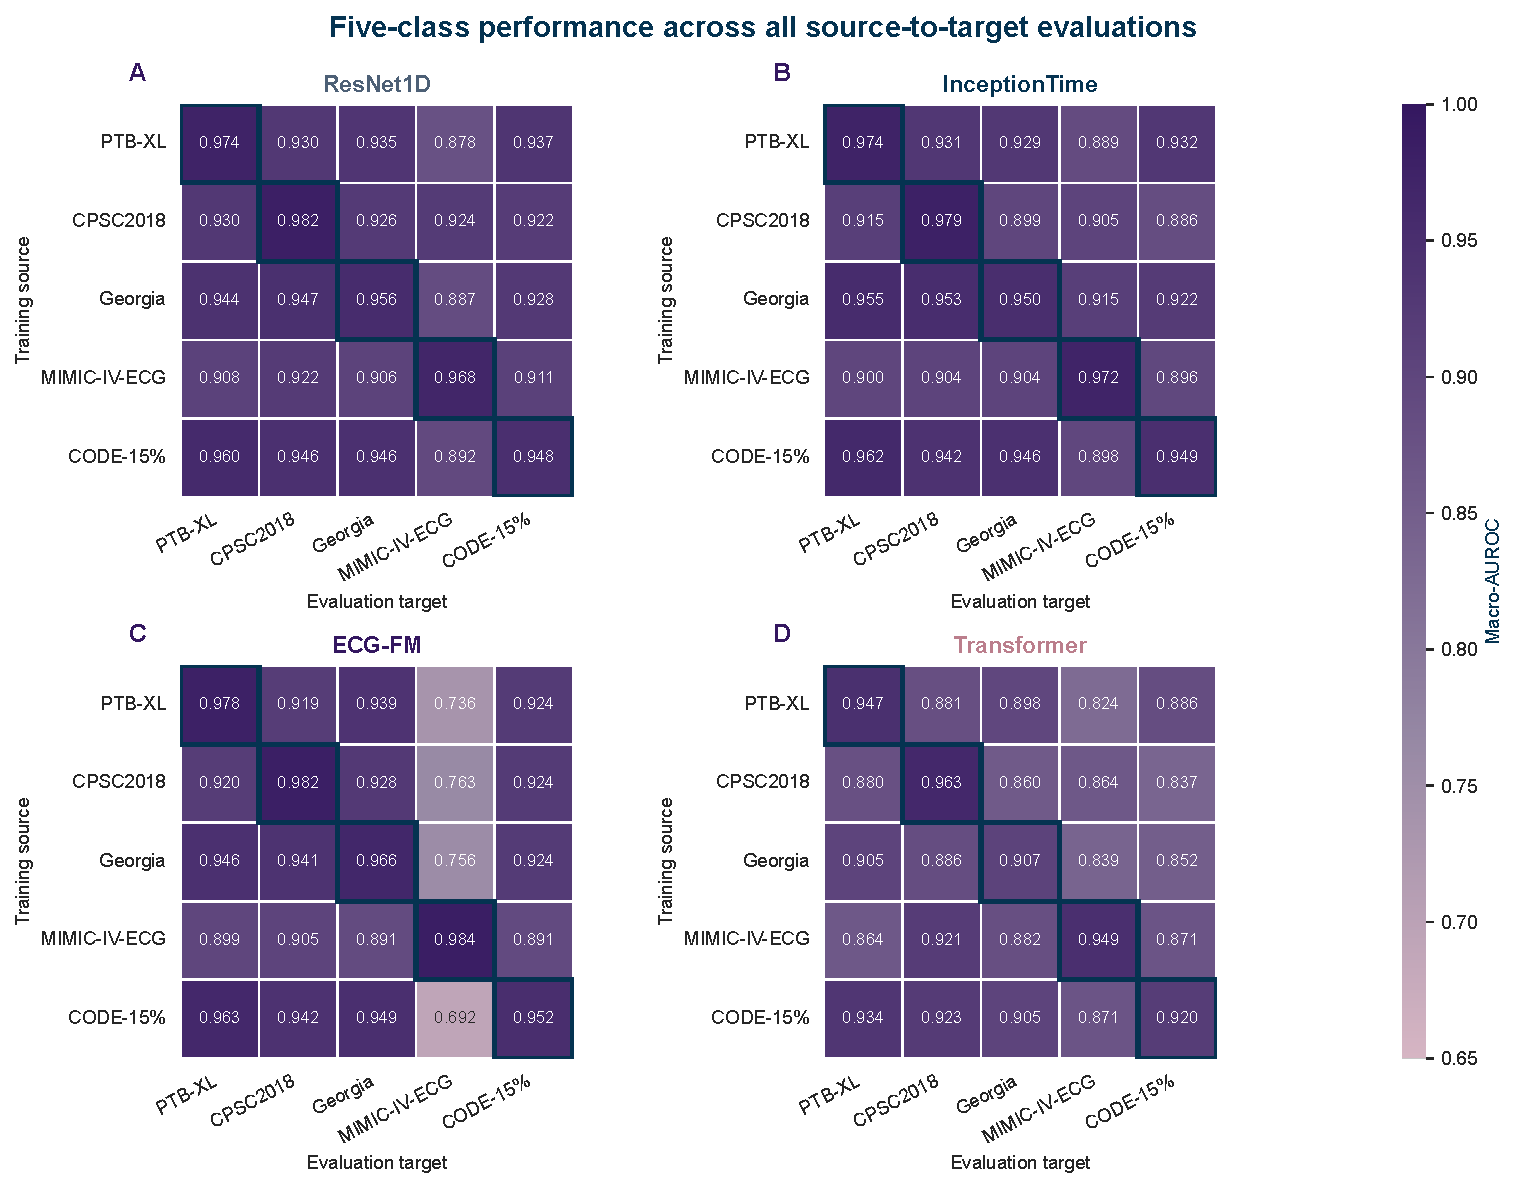
\includegraphics[width=\linewidth]{figures/fig2_four_model_heatmaps.pdf}
  \caption{Five-class macro-AUROC for all 100 source-to-target evaluations. Rows denote the training source and columns denote the evaluation target; outlined diagonal cells are in-distribution evaluations. The directional asymmetry and especially low MIMIC-IV-ECG target performance show why a single aggregate score is insufficient.}
  \label{fig:matrices}
\end{figure}

Pooling all four architectures' off-diagonal cells ($n=80$) into their shift-vector groups, a one-way ANOVA found no significant difference in raw gap magnitude between the groups ($F=0.14$, $p=0.87$). This suggests that the weighted attribution was influenced by the selected weights, so we treat it as a sensitivity analysis rather than an independently confirmed effect.

% TODO(results owner): Recompute the composite score and weight sweep from the audited ResNet1D matrix before restoring numerical composite rankings.
The composite score is retained as a secondary sensitivity analysis because its ranking depends on the selected population-, device-, and label-shift weights. Raw cross-dataset macro-AUROC and the unweighted generalization gap remain the primary results.

ECG-FM shows a greater decrease in performance when MIMIC-IV-ECG is the evaluation target (mean drop 0.236), compared with drops of 0.063--0.087 for the other three architectures, contrary to intuition given the pretraining overlap. This may be a result of MIMIC-IV-ECG's distinct machine-report-derived labeling pipeline rather than a true generalization failure, though this has not been independently verified.

\begin{figure}[t]
  \centering
  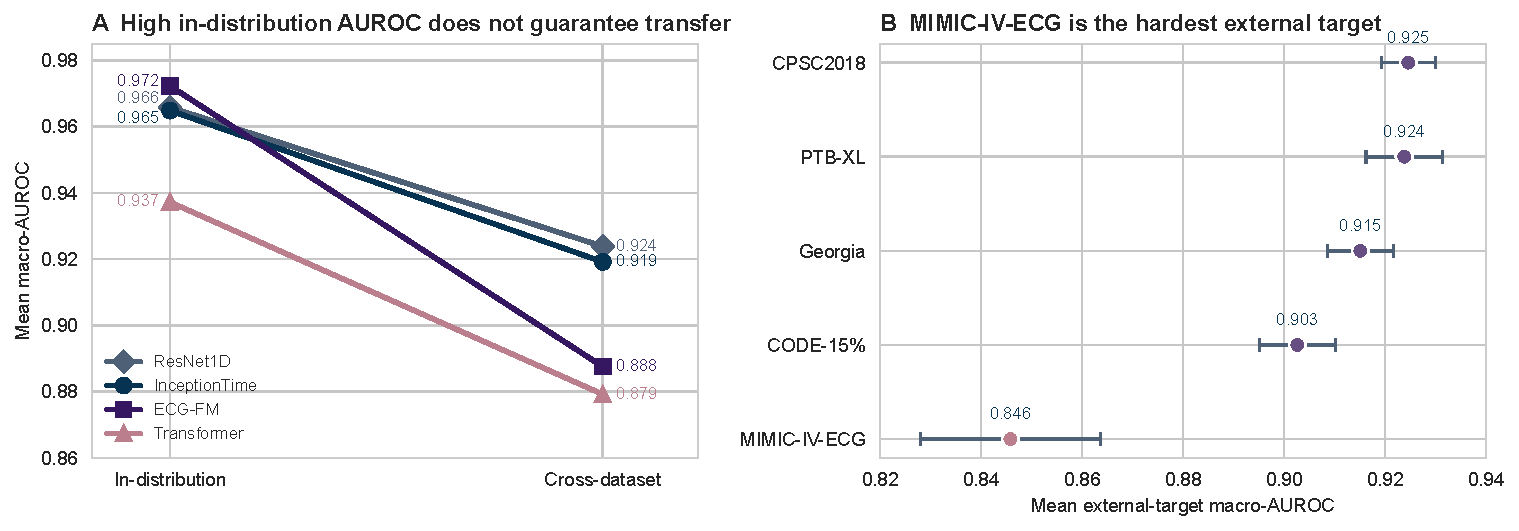
\includegraphics[width=\linewidth]{figures/fig3_generalization_summary.pdf}
  \caption{Generalization summary. \textbf{A}, model order changes between in-distribution and cross-dataset evaluation: ECG-FM leads in-distribution, whereas ResNet1D leads externally. \textbf{B}, averaged across models and external sources, MIMIC-IV-ECG is the hardest evaluation target. Error bars show the standard error across the contributing source-model cells.}
  \label{fig:summary}
\end{figure}

A post-hoc normal-versus-abnormal analysis across all four architectures reduced the matched-record average generalization gap from 0.049 to 0.038, a reduction of 22.5\%. The reductions were 1.8\% for ECG-FM, 41.8\% for InceptionTime, 43.7\% for ResNet1D, and 24.8\% for the Transformer. The alternative endpoint mappings changed absolute cross-dataset AUROC but did not change the model ranking, which remained ResNet1D, InceptionTime, ECG-FM, and Transformer (Figure~\ref{fig:sensitivity}).

\begin{figure}[t]
  \centering
  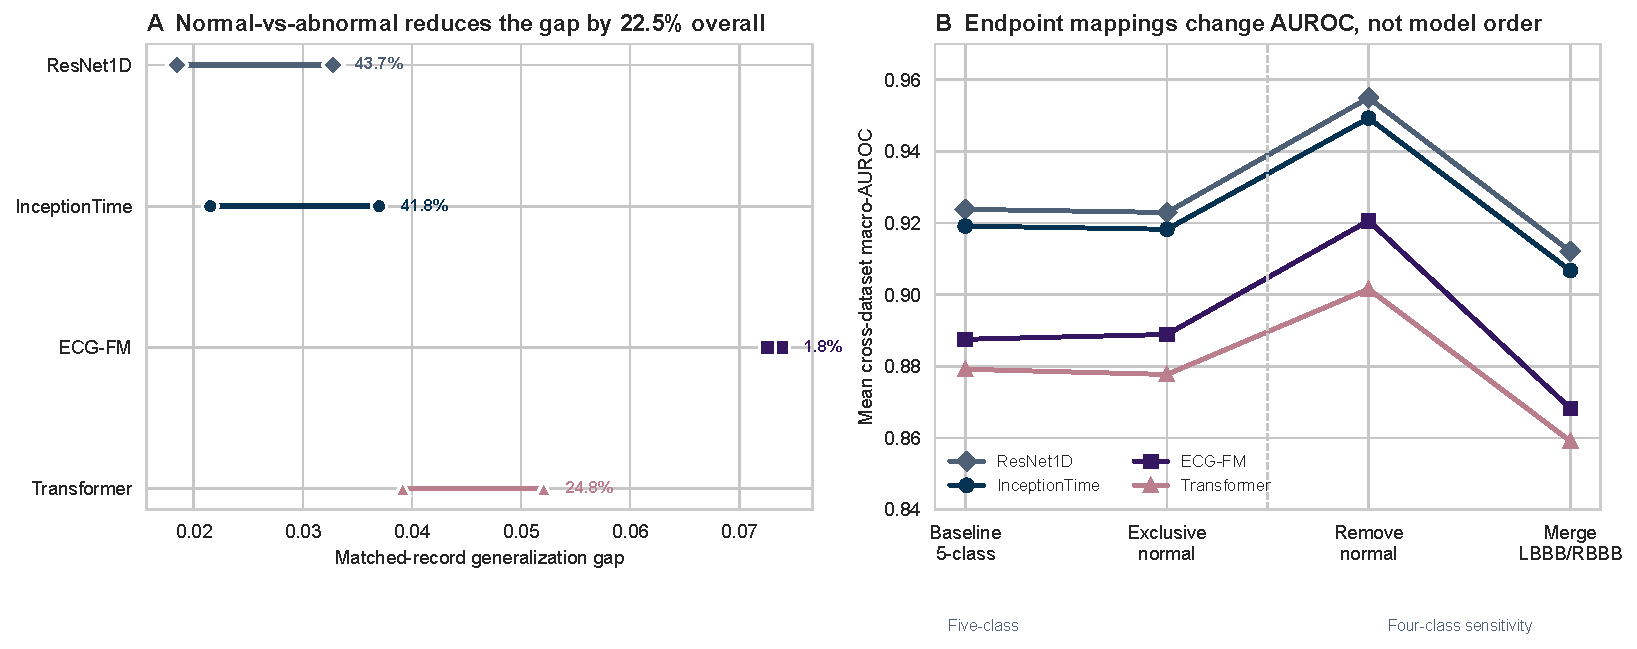
\includegraphics[width=\linewidth]{figures/fig4_revision_sensitivity.pdf}
  \caption{Post-hoc sensitivity analyses using fixed saved predictions. \textbf{A}, normal-versus-abnormal evaluation reduces the matched-record generalization gap overall, but the reduction varies by architecture. \textbf{B}, alternative endpoint mappings move absolute macro-AUROC but preserve the model order. The four-class variants are sensitivity diagnostics and are not directly comparable improvements over the five-class task.}
  \label{fig:sensitivity}
\end{figure}

\section{Discussion}

The results of the paper support the central idea for this benchmark that performing well on a held-out split from one dataset does not automatically indicate that the model will be able to generalize to ECG data collected elsewhere. ECG-FM had the highest average in-distribution AUROC of 0.972, but ResNet1D achieved the strongest cross-dataset AUROC at 0.924 and the smallest generalization gap of 0.042. InceptionTime followed at 0.919 with a gap of 0.046, while ECG-FM dropped to 0.888 and showed the largest gap at 0.085. These results show that in-distribution performance can be misleading when examining how robust a model might be outside its training data.

The target dataset also has bearing on the difficulty of generalization. Across the four architectures, MIMIC-IV-ECG had the lowest average external-target AUROC at 0.846. Correspondingly, PTB-XL had an average of 0.924, CPSC2018 had an average of 0.925, Georgia had an average of 0.915, and CODE-15\% had an average of 0.903. Some of the largest performance drops for ECG-FM occurred when MIMIC-IV-ECG was the target. However, the reverse transfers did not behave in the same way, showing that dataset shift is directional. Evaluating transfer from dataset A to B is therefore not equivalent to evaluating transfer from B to A.

The post-hoc normal-versus-abnormal analysis provides more direct evidence that differences in label definitions contribute to the generalization gap. Across all four architectures, the matched-record average gap decreased from 0.049 to 0.038, a 22.5\% reduction. However, the reduction varied across the four models, indicating that label granularity explains only part of the performance loss.

Because the datasets use different labeling systems, we adopted a shared label system that may not align every diagnosis perfectly. Label-schema differences appeared in many dataset pairs and also received the greatest weight in the scoring method. The attribution analysis should therefore be treated as a descriptive sensitivity analysis rather than a causal conclusion, since population, device, and labeling shifts often occur together and are difficult to isolate. The alternative endpoint mappings changed absolute cross-dataset AUROC but did not change the model ranking, suggesting that the comparison between architectures was stable.

\section{Limitations}

This benchmark only aligns five diagnostic classes, so it does not represent every abnormality contained in the original datasets. Mapping different coding systems into the same classes requires some judgment, and different mapping choices could change the results. The population, device, and label-schema shift categories are simplified measurements, and several shifts may occur at the same time. CPSC2018 is smaller than the other datasets, while inconsistent patient identifiers in some datasets limit our ability to guarantee patient-level separation in every split. Subsampling MIMIC-IV-ECG and CODE-15\% makes the experiments manageable but may leave out rare diagnoses or unusual waveform patterns. Finally, ECG-FM has previous exposure to MIMIC and PhysioNet data, and the study's retrospective AUROC-based evaluation does not directly measure calibration, fairness, clinical safety, or real-world patient outcomes. Because the revision analyses reused saved predictions, they could not recover source diagnoses excluded by the original mapping and should be interpreted as post-hoc sensitivity analyses rather than retrained ablations.

\section{Conclusion}

This study demonstrates that strong in-distribution ECG classification performance does not necessarily translate into robust cross-dataset generalization. Across five geographically and clinically diverse ECG datasets, every architecture experienced performance degradation when evaluated outside its training distribution, but the magnitude and direction of these drops varied substantially across models and dataset pairs. ECG-FM achieved the highest in-distribution AUROC, whereas ResNet1D achieved the strongest raw cross-dataset performance and smallest average generalization gap. The large variation between source-target pairs further suggests that dataset-specific differences cannot be adequately represented by a single aggregate notion of distribution shift. Together with the reduced cross-dataset gap in the post-hoc normal-versus-abnormal analysis, these findings indicate that differences in diagnostic labeling contribute meaningfully to apparent generalization failure. Overall, our results argue that ECG benchmarks should evaluate models across multiple external datasets and report both raw performance and sensitivity to benchmark design rather than relying solely on high performance within a single dataset.

\section{Future work}

Future work should extend the benchmark beyond the five diagnostic classes shared across the current datasets by developing richer harmonization strategies that preserve more of each dataset's original diagnostic information. Because the present shift-vector analysis cannot establish causality, controlled experiments could independently manipulate population characteristics, acquisition conditions, and label definitions to determine how much each factor directly contributes to cross-dataset degradation. Additional architectures and foundation models should also be evaluated to determine whether the robustness patterns observed here persist across newer ECG modeling approaches. Finally, future studies should evaluate uncertainty and prospective clinical performance in addition to AUROC, allowing cross-dataset robustness to be assessed in terms more directly relevant to real-world deployment.

\section{Responsible use statement}

This benchmark is intended for research evaluation and should not be used to make clinical decisions. Cross-dataset performance gaps, incomplete diagnostic coverage, retrospective labels, demographic imbalance, and uncertainty in label harmonization may produce unsafe or inequitable behavior in deployment. Any clinical use would require prospective external validation, calibration and subgroup analyses, clinician oversight, and governance appropriate to the intended setting. We release the mapping and sensitivity analyses to make these limitations auditable and to discourage unsupported claims of clinical generalization.

\section*{References}

\small

Perez Alday, E. A., et al. (2021). Classification of 12-lead ECGs: the PhysioNet/Computing in Cardiology Challenge 2020. \emph{Physiological Measurement}, 41(12), 124003.

Mobin, M. K., Islam, M. S., Barid, S. A., and Masum, M. (2025). Cardioformer: Advancing AI in ECG analysis with multi-granularity patching and ResNet. arXiv:2505.05538.

Wagner, P., et al. (2020). PTB-XL, a large publicly available electrocardiography dataset. \emph{Scientific Data}, 7, 154.

Wantlin, K., Wu, C., Huang, S.-C., et al. (2023). BenchMD: A benchmark for unified learning on medical images and sensors. arXiv:2304.08486.

% TODO before submission: Add complete Berger et al. (2026) and Zhou et al. (2026) entries.

\end{document}
